In this section we will only give an overview of all experiment results. The complete tables with all results are added in Appendix \ref{app:results}. In Table \ref{tab:results-summary}  we have summarized the results for some of the most interesting models. For the DDD, LDD and mc-flattened column, we give the best result that was found in the different experiment setups. 

\subsection{Time}
The timed results show that our symbolic solutions are slower for almost all models, compared to both \uppaal{} and the explicit state multi-core tool. Only for the small bocdp models we have a symbolic solution that is faster than \uppaal{}. 

One of the reasons we found was the high number of next-state calls. This is significantly higher than for the explicit-state tool as we partitioned the next-state function. For symbolic solutions this should be an advantage, as locality of transitions can be used. This same advantage should hold for the LDD solution we have, but the dependency matrices are too densely filled to give a real advantage. For the DDD solution we do not even make use of these localities, so there all advantages are lost. To confirm this hypothesis we also ran experiments without the partitioned next-state function. This gave for almost all models better results. The results differ from a small loss in speed to a speedup of a factor 10. This is still not enough to compete with \uppaal{}, but makes it possible to explore larger models within a given time-bound. 

Another problem seems to be the flattening of the DBM. This is an extra action that has to be executed in each next-state call, compared to the multi-core tool. This flattening is not a really expensive operation, it is only copying values, but it has to be executed a lot of times. For the DDD approach it is also necessary to close each DBM, as the DDD structure does not guarantee this. This is a more expensive operation and will also be executed in each next-state call. We implemented this in the language module, this closing is used for all experiments, so also for the experiments where it is not explicitly needed. This will also explain why the explicit state tool with subsumption is in most cases faster than the explicit state tool with flattened DBMs and without subsumption, even for models where subsumption will not have a real role, like the Viking models.

The last problem we see are the large state-vectors. This is mostly due to the quadratic size of the DBMs. For each of these variables a DDD level is created. As we have shown earlier, in some cases a lot of these levels will not have any impact on the zone represented. We can exploit this a little by setting these nodes to $(\infty,<)$, but the time-expensive function that does this has a larger impact on the timing results, which the benefits cannot outweigh. The diagram could make more use of this by skipping levels. This is not possible in our implementation as we only implicitly store the level of each node by its depth. 

\begin{landscape}
\begin{table}
    \begin{tabular}{|l|r|rr|rr|r|r|r|}
    \hline
     Model      & Discrete states & DDD     & ~     & LDD     & ~     & mc-flattened & mc-original & Uppaal \\
    ~           & ~               & \#nodes & time  & \#nodes & time  & time         & time        & time   \\ \hline
    fischer6    & 16320           & 15156   & 481.9 & 85041   & 48.3  & 19.2         & 0.4         & 0.0    \\
    critRegion4 & 6629            & 55890   & 46.3  & 100006  & 39.5  & 24.3         & 0.5         & 0.1    \\
    Critical4   & -               & -       & TO    & -       & TO    & 1.1          & 0.5         & 0.6    \\
    CSMACD8     & 10515           & 96098   & 1.9   & 321001  & 7.3   & 6.9          & 0.5         & 0.1    \\
    Viking12    & 241662          & 342     & 17.6  & 342     & 18.7  & 10.4         & 0.7         & 1.0    \\
    Lynch5      & 228579          & 49430   & 34.2  & 112397  & 120.0 & 50.0         & 0.3         & 0.0    \\
    bocdp       & 33              & 487     & 0.1   & 355     & 0.2   & 0.2          & 0.0         & 0.2    \\
    bocdpFIXED  & 33              & 488     & 0.2   & 427     & 0.2   & 0.1          & 0.0         & 0.3    \\
    bando       & 33              & 488     & 0.2   & 425     & 0.2   & 0.1          & 0.0         & 0.3    \\
    Milner8     & 128             & 11012   & 0.4   & 30887   & 1.2   & 1.4          & 0.1         & 0.0    \\
    hddi10      & 86              & -       & TO    & 454246  & 93.3  & 43.1         & 0.0         & 0.0    \\ \hline
    \end{tabular}
\caption{Summarized table of results with number of discrete states, nodes and time in seconds}
\label{tab:results-summary}
\end{table}
\end{landscape}

\subsection{Memory}
We have not measured memory usage. A good symbolic solution will use a lot of memory for caching when it is available. Comparing this to other solutions which use less caching will not be representative. We do compare the number of nodes between the different solutions. 

For most models the best DDD solutions use less nodes than the best LDD solution. This is what we expected as local reductions on clocks can be made. For the smallest models the LDD sometimes gives less nodes for some reorderings. These models have such low number of clocks that no reductions can be made yet. The bocdp and bando models are the largest models which have a lower LDD than DDD representation. These models have quite a high number of discrete variables with a low number of clocks. For most larger models the LDD solution without reordering is smaller than with reordering. This is probably due to the densely filled matrices, so no good reorderings can be created from them.

There is a difference between the number of nodes for the normal BFS and the BFS without minus. This is possible because we do not use a canonical form of DDDs. Most results show a higher number of nodes for the runs with the minus. In Figure \ref{fig:fragmentation} we show an example of how this can happen. We assume all zones in the figures belong to the same set of locations. In Figure \ref{fig:vis_zone} we have the zone that is already visited. Now a new state with the zone in Figure \ref{fig:cur_zone} is discovered. If the minus is not used, successors of this state are directly generated from the set of locations and this zone. If the minus is used the first zone will first be subtracted before successors are generated. The result of the subtraction is shown in Figure \ref{fig:after_minus_zone}. This is not a convex zone, so a DDD with multiple paths is needed. From this state also other successors can be generated, possibly needing more nodes to be represented. If the newly generated states are then unioned with the visited set the result can again have more nodes than the version without minus. The less fractioned zones in the current set can also have implications on the time results, as less work in the next-state function is needed. On the other hand the next-state function can also need extra time, as some states would otherwise have completely been removed from the current set, and no work for that states would need to be done. 

\begin{figure}[h]

\begin{subfigure}[b]{\textwidth}
\centering
\begin{adjustbox}{max totalheight=.3\textheight}
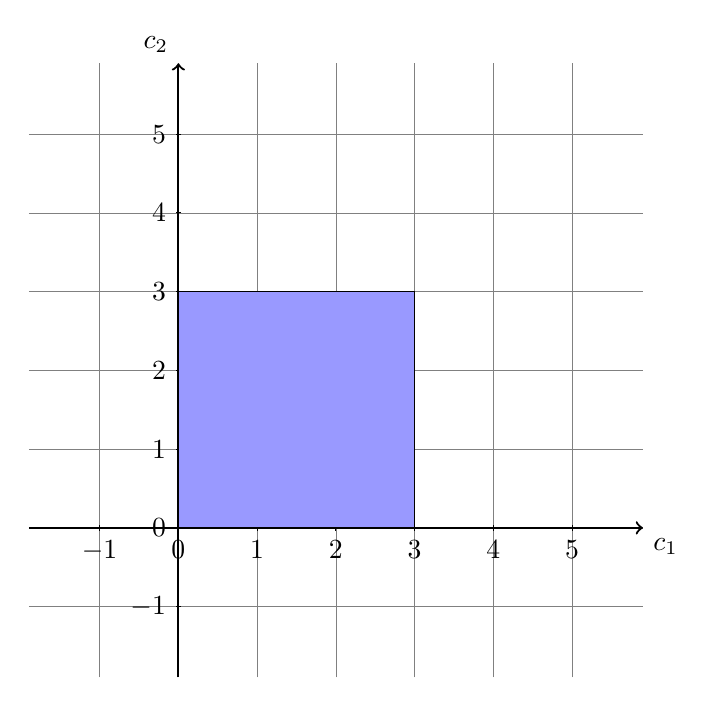
\begin{tikzpicture}

\draw[step=1cm,gray,very thin] (-1.9,-1.9) grid (5.9,5.9);

%\shadedraw[inner color=blue,outer color=red, draw=black] (0,0) rectangle (4,4);

\draw[thick,->] (-1.9,0) -- (5.9,0) node[anchor=north west] {$c_1$};
\draw[thick,->] (0,-1.9) -- (0,5.9) node[anchor=south east] {$c_2$};

\foreach \x in {-1,0,1,2,3,4,5}
    \draw (\x cm,1pt) -- (\x cm,-1pt) node[anchor=north] {$\x$};
\foreach \y in {-1,0,1,2,3,4,5}
    \draw (1pt,\y cm) -- (-1pt,\y cm) node[anchor=east] {$\y$};
    
\filldraw[fill=blue!40!white, draw=black] (0,0) rectangle (3,3);

\end{tikzpicture}
\end{adjustbox}
\caption{Visited Zone}
\label{fig:vis_zone}
\end{subfigure}



\begin{subfigure}[b]{\textwidth}
\centering
\begin{adjustbox}{max totalheight=.3\textheight}
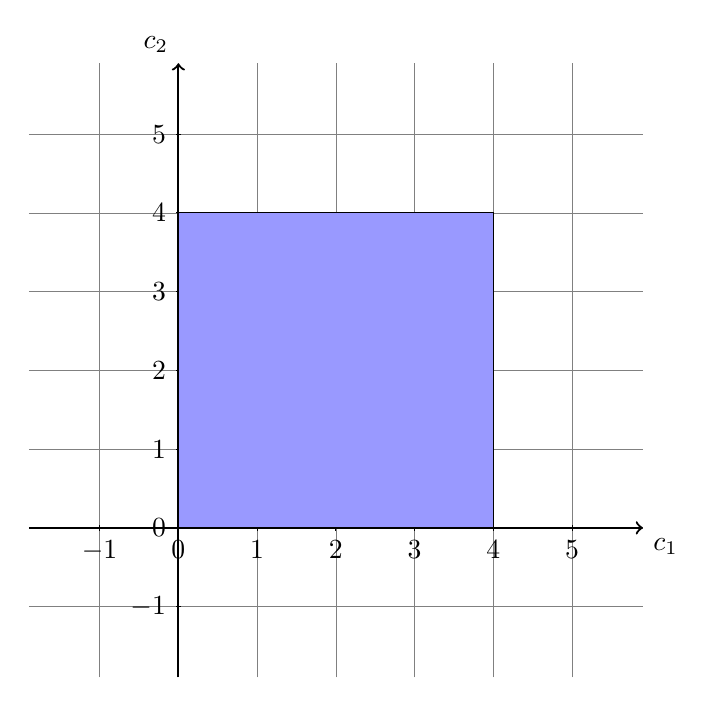
\begin{tikzpicture}
\draw[step=1cm,gray,very thin] (-1.9,-1.9) grid (5.9,5.9);

%\shadedraw[inner color=blue,outer color=red, draw=black] (0,0) rectangle (4,4);

\draw[thick,->] (-1.9,0) -- (5.9,0) node[anchor=north west] {$c_1$};
\draw[thick,->] (0,-1.9) -- (0,5.9) node[anchor=south east] {$c_2$};

\foreach \x in {-1,0,1,2,3,4,5}
    \draw (\x cm,1pt) -- (\x cm,-1pt) node[anchor=north] {$\x$};
\foreach \y in {-1,0,1,2,3,4,5}
    \draw (1pt,\y cm) -- (-1pt,\y cm) node[anchor=east] {$\y$};
    
\filldraw[fill=blue!40!white, draw=black] (0,0) rectangle (4,4);

\end{tikzpicture}
\end{adjustbox}
\caption{Current Zone}
\label{fig:cur_zone}
\end{subfigure}


\begin{subfigure}[b]{\textwidth}
\centering
\begin{adjustbox}{max totalheight=.3\textheight}
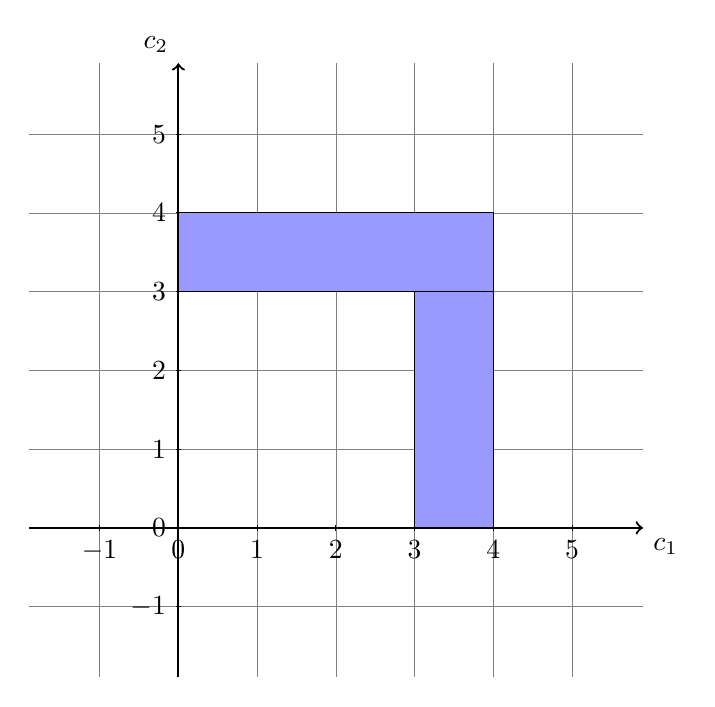
\begin{tikzpicture}
\draw[step=1cm,gray,very thin] (-1.9,-1.9) grid (5.9,5.9);

%\shadedraw[inner color=blue,outer color=red, draw=black] (0,0) rectangle (4,4);

\draw[thick,->] (-1.9,0) -- (5.9,0) node[anchor=north west] {$c_1$};
\draw[thick,->] (0,-1.9) -- (0,5.9) node[anchor=south east] {$c_2$};

\foreach \x in {-1,0,1,2,3,4,5}
    \draw (\x cm,1pt) -- (\x cm,-1pt) node[anchor=north] {$\x$};
\foreach \y in {-1,0,1,2,3,4,5}
    \draw (1pt,\y cm) -- (-1pt,\y cm) node[anchor=east] {$\y$};
    
\filldraw[fill=blue!40!white, draw=black] (0,3) rectangle (4,4);
\filldraw[fill=blue!40!white, draw=black] (3,0) rectangle (4,3);

\end{tikzpicture}
\end{adjustbox}
\caption{After Minus}
\label{fig:after_minus_zone}
\end{subfigure}

\caption{Minus fragmentation}
\label{fig:fragmentation}
\end{figure}

The DBM reduction does not give the results we aimed for. For most models exploration is faster without the reduction. This is due to the expensive algorithm that the reduction is. Also the reduction of the number of nodes is not what we hoped for. Most models get more nodes when the reduction is turned on. The reduction can however still become usefull if we go to a canonical DDD representation. 

